\documentclass[a4paper, 12pt]{article}

\def\languages{french, english}

%%%%%%%%%%%%%%%%%%% Libraries

%%%%%%%%%% Packages

\usepackage[
backend=biber,
style=numeric-comp,
sorting=none,
maxbibnames=99
]{biblatex}

\newgeometry{margin = 2.5cm}
\makeatletter
\begin{titlepage}
	\begin{minipage}[t][0.425\textheight][t]{\textwidth}
		\begin{center}
		    \ifx\toptitle\undefined
    		    \vfill
    		    \ifx\logopath\undefined
    		    \else
    			    \includegraphics[height=0.2125\textheight]{\logopath}
    			\fi
    		\else
    		    \ifx\logopath\undefined
    		    \else
    			    \includegraphics[height=0.15\textheight]{\logopath}
    			\fi
    			\vfill
    			{\huge \textsc{\toptitle}}
			\fi
			\vfill
		\end{center}
	\end{minipage}
	\vfill
	\begin{minipage}{\textwidth}
		\hspace{0.5em}
		\begin{mdframed}[linewidth = 2pt, innertopmargin = 1em, innerbottommargin = 1em, leftline = false, rightline = false]
			\begin{center}
				{\huge \bfseries \@title}
			\end{center}
		\end{mdframed}
		\hspace{0.5em}
	\end{minipage}
	\vfill
	\begin{minipage}[b][0.425\textheight][t]{\textwidth}
			\ifx\subtitle\undefined
			\else
			    \vspace{-0.5em}
			    \begin{center}
				    {\LARGE \subtitle}
				\end{center}
			\fi
			\vfill
			\ifx\rightauthor\undefined
			    \begin{center}
			        \ifx\authorhead\undefined
			        \else
		                {\large\it \authorhead\\[0.5em]}
		            \fi
			        {\large \@author}
			    \end{center}
			\else
			    \begin{minipage}[t]{0.5\textwidth}
			        \begin{flushleft}
			            \ifx\authorhead\undefined
			            \else
			                {\large\it \authorhead\\[0.5em]}
			            \fi
				        {\large \@author}
				    \end{flushleft}
				\end{minipage}
				\begin{minipage}[t]{0.5\textwidth}
				    \begin{flushright}
				        \ifx\rightauthorhead\undefined
			            \else
			                {\large\it \rightauthorhead\\[0.5em]}
			            \fi
				        {\large \rightauthor}
				    \end{flushright}
				\end{minipage}
			\fi
			\vfill
			\begin{center}
			    \ifx\context\undefined
			    \else
			        {\large \context \\[0.5em]}
			    \fi
			    {\large \@date}
			\end{center}
	\end{minipage}
\end{titlepage}
\makeatother
\restoregeometry
%%%%%%%%%% Packages

\usepackage{float}
\usepackage[skip=1em]{caption}
\usepackage{subcaption}

\usepackage{array}
\usepackage{multirow}
\usepackage{multicol}

%%%%%%%%%% Features

%%%%% Settings

\renewcommand{\arraystretch}{1.2}

%%%%% Commands

\newcommand\noskipcaption[1]{\caption{#1}\vspace{-1em}}
\newcommand\noskipcaptionstar[1]{\caption*{#1}\vspace{-1em}}

%%%%%%%%%% Packages

\usepackage{inconsolata}
\usepackage{listings}

%%%%%%%%%% Features

%%%%% Commands

\newcommand{\Nstyle}[1]{
    \lstdefinestyle{N#1}{
        style=#1,
        %%%%%
        numbers=left
    }
}

\newcommand{\tbFstyle}[1]{
    \lstdefinestyle{tbF#1}{
        style=#1,
        %%%%%
        frame=tb
    }
}

\newcommand{\Fstyle}[1]{
    \lstdefinestyle{F#1}{
        style=#1,
        %%%%%
        frame=single,
        framesep=0em,
        rulesep=0em,
        xleftmargin=0.75em,
        xrightmargin=0.75em,
        framexleftmargin=0.75em,
        framexrightmargin=0.75em,
        framextopmargin=0.5em,
        framexbottommargin=0.5em,
        %%%%%
        numbersep=1.25em
    }
}

\newcommand{\NtbFstyle}[1]{
    \tbFstyle{#1}
    \Nstyle{tbF#1}
}

\newcommand{\NFstyle}[1]{
    \Fstyle{#1}
    \lstdefinestyle{NF#1}{
        style=f#1,
        %%%%%
        xleftmargin=2.75em,
        framexleftmargin=2.75em,
        %%%%%
        numbers=left,
        numbersep=1em
    }
}

%%%%% Styles

\lstdefinestyle{default}{
    breaklines=true,
    breakatwhitespace=true,
    columns=fixed,
	extendedchars=true,
    upquote=true,
	tabsize=4,
    %%%%%
    framerule=0.66pt,
    captionpos=b,
	%%%%%
    basicstyle=\footnotesize\ttfamily,
    numberstyle=\footnotesize\ttfamily,
    showstringspaces=false
}
\Nstyle{default}
\NFstyle{default}
\NtbFstyle{default}

\lstdefinestyle{monokai}{
    style=Fdefault,
    %%%%%
    backgroundcolor=\color[HTML]{272822},
    framerule=0em,
    %%%%%
    basicstyle=\footnotesize\ttfamily\color[HTML]{f8f8f2},
    numberstyle=\footnotesize\ttfamily\color[HTML]{272822},
    commentstyle=\color[HTML]{75715e},
    keywordstyle=[1]{\color[HTML]{f92672}},
    keywordstyle=[2]{\color[HTML]{A6E22E}},
    keywordstyle=[3]{\color[HTML]{ae81ff}},
    stringstyle=\color[HTML]{e6db74},
    %%%%%
    % otherkeywords={!,.,+,-,*,/,=,<,>,^,|,\&,OR,AND}
}

\lstdefinestyle{Nmonokai}{
    style=monokai,
    %%%%%
    xleftmargin=2.75em,
    framexleftmargin=2.75em,
    %%%%%
    numbers=left,
    numberstyle=\footnotesize\ttfamily\color[HTML]{f8f8f2},
    numbersep=1em
}

\lstdefinestyle{c}{
    language=C,
    style=default,
    %%%%%
    commentstyle=\color[HTML]{228B22},
    keywordstyle=\color[HTML]{0000FF},
    stringstyle=\color[HTML]{A020F0},
    emphstyle=\color[HTML]{0000FF},
    %%%%%
    emph={}
}

\lstdefinestyle{cpp}{
    language=C++,
    style=default,
    %%%%%
    commentstyle=\color[HTML]{228B22},
    keywordstyle=\color[HTML]{0000FF},
    stringstyle=\color[HTML]{A020F0},
    emphstyle=\color[HTML]{0000FF},
    %%%%%
    emph={std}
}

\lstdefinestyle{matlab}{
    language=matlab,
    style=default,
    %%%%%
    basicstyle=\footnotesize\fontfamily{pcr}\selectfont,
    numberstyle=\footnotesize\fontfamily{pcr}\selectfont,
    commentstyle=\color[HTML]{228B22},
    keywordstyle=\color[HTML]{0000FF},
    stringstyle=\color[HTML]{A020F0},
    emphstyle=\color[HTML]{0000FF},
    %%%%%
    emph={clearvars}
}

\lstdefinestyle{python}{
    language=python,
    style=default,
    %%%%%
    commentstyle=\color[RGB]{221,0,0},
    keywordstyle=[1]{\color[RGB]{255,119,0}},
    keywordstyle=[2]{\color[RGB]{144,0,144}},
    stringstyle=\color[RGB]{0,170,0},
    emphstyle=\color[RGB]{255,119,0},
    %%%%%
    emph={}
}

\lstdefinestyle{java}{
    language=java,
    style=default,
    %%%%%
    commentstyle=\color[HTML]{228B22},
    keywordstyle=\color[HTML]{0000FF},
    stringstyle=\color[HTML]{A020F0},
    emphstyle=\color[HTML]{0000FF},
    %%%%%
    emph={}
}

%%%%%%%%%% Packages

\usepackage{amsmath}
\usepackage{amssymb}
\usepackage{bm}
\usepackage{esint}
\usepackage[makeroom]{cancel}

%%%%%%%%%% Features

%%%%% Macros

\newcommand{\rbk}[1]{\left(#1\right)}
\newcommand{\cbk}[1]{\left\{#1\right\}}
\newcommand{\sbk}[1]{\left[#1\right]}
\newcommand{\abs}[1]{\left|#1\right|}
\newcommand{\norm}[1]{\left\|#1\right\|}

\newcommand{\fact}[1]{#1!}
\newcommand{\e}[1]{\mathbf{e}_{#1}}
\newcommand{\deriv}{\mathrm{d}}
\DeclareMathOperator{\tr}{tr}

\def\Rl{\mathbb{R}}
\def\Cx{\mathbb{C}}
\def\Na{\mathbb{N}}
\def\Zi{\mathbb{Z}}

%%%%%%%%%% Packages

\usepackage{amsthm}
\usepackage{thmtools}

%%%%%%%%%% Features

%%%%% Settings

\makeatletter
\define@key{thmdef}{mdthm}[{}]{
	\thmt@trytwice{\def\thmt@theoremdefiner{\mdtheorem[#1]}}{}}
\makeatother

\begingroup
\makeatletter
\@for\theoremstyle:=plain,definition,remark\do{
	\expandafter\g@addto@macro\csname th@\theoremstyle\endcsname{
		\addtolength\thm@preskip\parskip
	}
}
\endgroup

\renewcommand{\qedsymbol}{$\blacksquare$}

% language

\ifx\lgthm\undefined
	\def\lgthm{Theorem}
	\def\lgprf{Proof}
	\def\lglem{Lemma}
	\def\lgprop{Proposition}
	\def\lgdefn{Definition}
	\def\lghyp{Hypothesis}
	\def\lgmeth{Method}
	\def\lgquest{Question}
	\def\lgansw{Answer}
	\def\lgexpl{Example}
	\def\lgrmk{Remark}
	\def\lgnote{Note}
	\def\lgtip{Tip}
\fi

%%%%% Commands

\newcommand\qedadd{\pushQED{\qed}\popQED}

%%%%% Environments

\theoremstyle{plain}
\newtheorem{thm}{\lgthm}
\newtheorem{lem}[thm]{\lglem}
\newtheorem{prop}[thm]{\lgprop}

\theoremstyle{definition}
\newtheorem{defn}{\lgdefn}
\newtheorem{hyp}{\lghyp}
\newtheorem{meth}{\lgmeth}
\newtheorem{quest}{\lgquest}

\theoremstyle{remark}
\newtheorem{answ}{\lgansw}[quest]
\newtheorem{expl}{\lgexpl}
\newtheorem*{rmk}{\lgrmk}
\newtheorem*{note}{\lgnote}
\newtheorem*{tip}{\lgtip}

% framed

\mdfdefinestyle{thicc}{
	nobreak=true,
	skipabove=\topskip,
	skipbelow=\topskip,
	innerleftmargin=0.5em,
	innerrightmargin=0.5em,
	innerbottommargin=0.5em,
	innertopmargin=0.5em,
	linewidth=0.25em,
	roundcorner=0.15em,
	linecolor=black!10,
	frametitlebackgroundcolor=black!10,
	theoremseparator={.}
}

\declaretheorem[mdthm={style=thicc, linecolor=red!20, frametitlebackgroundcolor=red!20}, sibling=thm, name=\lgthm]{framedthm}
\declaretheorem[mdthm={style=thicc, linecolor=red!20, frametitlebackgroundcolor=red!20}, sibling=thm, name=\lglem]{framedlem}
\declaretheorem[mdthm={style=thicc, linecolor=blue!20, frametitlebackgroundcolor=blue!20}, sibling=thm, name=\lgprop]{framedprop}
\declaretheorem[mdthm={style=thicc, nobreak=false}, parent=thm, name=\lgprf]{framedprf}

\declaretheorem[mdthm={style=thicc, linecolor=black!20!green!20, frametitlebackgroundcolor=black!20!green!20}, sibling=defn, name=\lgdefn]{frameddefn}
\declaretheorem[mdthm={style=thicc, linecolor=blue!20, frametitlebackgroundcolor=blue!20}, sibling=hyp, name=\lghyp]{framedhyp}
\declaretheorem[mdthm={style=thicc}, name=\lgmeth]{framedmeth}
\declaretheorem[mdthm={style=thicc, linecolor=orange!20, frametitlebackgroundcolor=orange!20}, sibling=quest, name=\lgquest]{framedquest}

\declaretheorem[mdthm={style=thicc, nobreak=false}, sibling=answ, name=\lgansw]{framedansw}
\declaretheorem[mdthm={style=thicc, nobreak=false}, sibling=expl, name=\lgexpl]{framedexpl}

%%%%%%%%%% Packages

\usepackage{siunitx}

%%%%%%%%%% Features

%%%%% Settings

\ifx\decimalsign\undefined
\else
    \sisetup{output-decimal-marker = \decimalsign}
\fi


%%%%%%%%%%%%%%%%%%% Titlepage

\def\logopath{resources/pdf/logo-uliege.pdf}
\def\toptitle{University of Liège}
\title{Activity prediction for chemical compounds}
\def\subtitle{Introduction to machine learning}
%\def\authorhead{Author}
\author{
    Maxime \textsc{Meurisse} (20161278)\\
    François \textsc{Rozet} (20161024)\\
    Valentin \textsc{Vermeylen} (20162864)\\
}
%\def\rightauthorhead{}
%\def\rightauthor{}
\def\context{MSc in Computer Science and Engineering}
\date{Academic year 2019-2020}

%%%%%%%%%%%%%%%%%%% Options

\fancyhead[R]{}
\geometry{paper=a4paper,margin=2.5cm}
\addbibresource{references.bib}

%%%%%%%%%%%%%%%%%%% Additional packages

\usepackage{wrapfig}
\usepackage{colortbl}

%%%%%%%%%%%%%%%%%%% Document

\begin{document}
    % ----- Title page ----- %
	\newgeometry{margin = 2.5cm}
\makeatletter
\begin{titlepage}
	\begin{minipage}[t][0.425\textheight][t]{\textwidth}
		\begin{center}
		    \ifx\toptitle\undefined
    		    \vfill
    		    \ifx\logopath\undefined
    		    \else
    			    \includegraphics[height=0.2125\textheight]{\logopath}
    			\fi
    		\else
    		    \ifx\logopath\undefined
    		    \else
    			    \includegraphics[height=0.15\textheight]{\logopath}
    			\fi
    			\vfill
    			{\huge \textsc{\toptitle}}
			\fi
			\vfill
		\end{center}
	\end{minipage}
	\vfill
	\begin{minipage}{\textwidth}
		\hspace{0.5em}
		\begin{mdframed}[linewidth = 2pt, innertopmargin = 1em, innerbottommargin = 1em, leftline = false, rightline = false]
			\begin{center}
				{\huge \bfseries \@title}
			\end{center}
		\end{mdframed}
		\hspace{0.5em}
	\end{minipage}
	\vfill
	\begin{minipage}[b][0.425\textheight][t]{\textwidth}
			\ifx\subtitle\undefined
			\else
			    \vspace{-0.5em}
			    \begin{center}
				    {\LARGE \subtitle}
				\end{center}
			\fi
			\vfill
			\ifx\rightauthor\undefined
			    \begin{center}
			        \ifx\authorhead\undefined
			        \else
		                {\large\it \authorhead\\[0.5em]}
		            \fi
			        {\large \@author}
			    \end{center}
			\else
			    \begin{minipage}[t]{0.5\textwidth}
			        \begin{flushleft}
			            \ifx\authorhead\undefined
			            \else
			                {\large\it \authorhead\\[0.5em]}
			            \fi
				        {\large \@author}
				    \end{flushleft}
				\end{minipage}
				\begin{minipage}[t]{0.5\textwidth}
				    \begin{flushright}
				        \ifx\rightauthorhead\undefined
			            \else
			                {\large\it \rightauthorhead\\[0.5em]}
			            \fi
				        {\large \rightauthor}
				    \end{flushright}
				\end{minipage}
			\fi
			\vfill
			\begin{center}
			    \ifx\context\undefined
			    \else
			        {\large \context \\[0.5em]}
			    \fi
			    {\large \@date}
			\end{center}
	\end{minipage}
\end{titlepage}
\makeatother
\restoregeometry
	
	% ----- Introduction ----- %
	\section{Introduction}
The project is organized as a competition between different teams on the Kaggle platform. As mentioned on this website, it consists of using (supervised) learning techniques to design a model able to predict the activity of a chemical compound (described by its molecular structure). The main goal is about {\it determining the ability for a chemical compound to inhibit HIV replication}. \cite{kaggle-iml2019}

Since the prediction associated with each molecule is a boolean (the molecules inhibit HIV replication or not), we tried classification methods. We used the methods seen during the course, but also other methods found in scientific papers or websites. We also took inspiration in this \href{https://scikit-learn.org/stable/tutorial/machine_learning_map/index.html}{scikit-learn flowchart} to guide our tests.

The main classifiers we focus about were the \emph{K-Neighbors Classifier}, \emph{Multilayer Perceptron}, \emph{Random Forest Classifier}, \emph{Support Vector Machine} and combinations of those using \emph{Ensemble} and handcrafted methods.

First of all, we tested each method individually without changing any parameters to get an idea of their performance (cf. section \ref{sec:AUC}). Then we tried to optimize the parameters of each one by iteratively applying them on the learning set and estimating their accuracy. Since the results weren't satisfying enough both with for local estimation and for the kaggle platform, we had the idea of combining them which lead better results.

Apart from the actual classifier algorithm, we also tried several fingerprint representations of the SMILES molecules. For example, we tried the following : \emph{Morgan}, \emph{RDKFingerprint} (Daylight-like), \emph{Avalon}, \emph{MACCS} fingerprints and a few others. Each of them have parameters that we tried to tweak for the better. However, we only realized that there were different fingerprints near the end of our journey which did not left us with a lot of time to experiment with them.

	
	% ----- Data pre-processing ----- %
	\section{Data pre-processing}
In order to train our models, we received a training set consisting of \num{15939} chemical compounds with their corresponding activity. Each chemical compound is described under the SMILES format (a line notation for the chemical structure of molecules). However, this format is difficult to use as it is by our models\footnote{Afterwards, we think that we could have tried text analysis algorithms.}. We therefore transformed the SMILES into binary fingerprints (cf. section \ref{sec:fingerprint}), i.e. vector of zeros and ones describing features.

Most of the time these fingerprints are sparse, therefore it is possible that one of the feature is the \emph{same} for all molecules. Therefore we applied a variance threshold \cite{scikit-variance-threshold} to remove all features whose variances are null.

	
	% ----- Estimation of the AUC ----- %
	\section{Estimation of the AUC}\label{sec:AUC}
To evaluated the accuracy of our models we used the ROC AUC metric (area under the ROC curve) available in the scikit-learn library \cite{scikit-roc-auc-score} combined with a random permutation cross-validator \cite{scikit-shufflesplit}.

The latter works as follow : a random permutation of the learning set is computed. The model is trained on a $1 - x$ portion of the permutation and used to predict the class of the remaining $x$ portion. Then the AUC score is computed using the prediction probabilities and the actual classes. This is repeated $n$ times. Finally, the $n$ gathered scores are averaged.

In contrast to the classic \emph{KFold} cross-validator, this one dissociates the number of splits ($n$) and the test size ($x$). In our case we chose $x = 0.25$ and $n = 5$.

The comparison between the estimated AUC and the actual (private) AUC will be conducted in section \ref{sec:performance}.

	
	% ----- Models ----- %
	\section{Models}
As said in the introduction we first tested the k-neighbors classifier (KNN), multilayer perceptron (MLP), random forest classifier (RFC) and support vector machine (SVM) algorithms individually with the original Morgan fingerprint. We also tried decision tree classifier (DTC) and linear discriminant analysis (LDA) but they were a lot worse than the others.

The estimations gravitated around \SI{74}{\percent}, but when we submitted these algorithms, the results were quite poor ($\sim$\SI{71}{\percent}) in comparison. We then realized that using the \texttt{useFeature = True} parameter significantly increased the score for both our estimations and Kaggle scores. Since we don't know much about organic chemistry, the consequences of this parameter are kind of blurry in our mind. Yet from what we understood, when set to \texttt{True}, the algorithm will detect feature-based invariants (predefined patterns) within the molecule \cite{scikit-morgan-features}.

At the same time, we noticed the parameters \texttt{nBits} (the number of bits in the bit vector) and \texttt{radius}. But, since we didn't want our scripts to run for too long, we didn't increase the number of bits until the end of our parameters testing phase, which was unfortunate as increasing that parameter usually provided better results (but induced computation times that were much longer).

In the following, if it not precised, the fingerprint used is Morgan, the number of bits $128$, the radius $2$ and the parameter \texttt{useFeature} is \texttt{True}.

\subsection{K-Neighbors classifier}

The parameter influencing the score of this method are the number of neighbors considered (\texttt{n\_neighbors}), the weight associated to each neighbor w.r.t. the distance (\texttt{weights}) and the distance metric used (\texttt{metric}). For weights, we tried two options : independent of the distance and proportional to the inverse of the distances. For metrics, we tried every bit vector metrics available \cite{scikit-distance-metrics}.

\begin{figure}[h]
    \begin{subfigure}{0.49\textwidth}
        \centering
        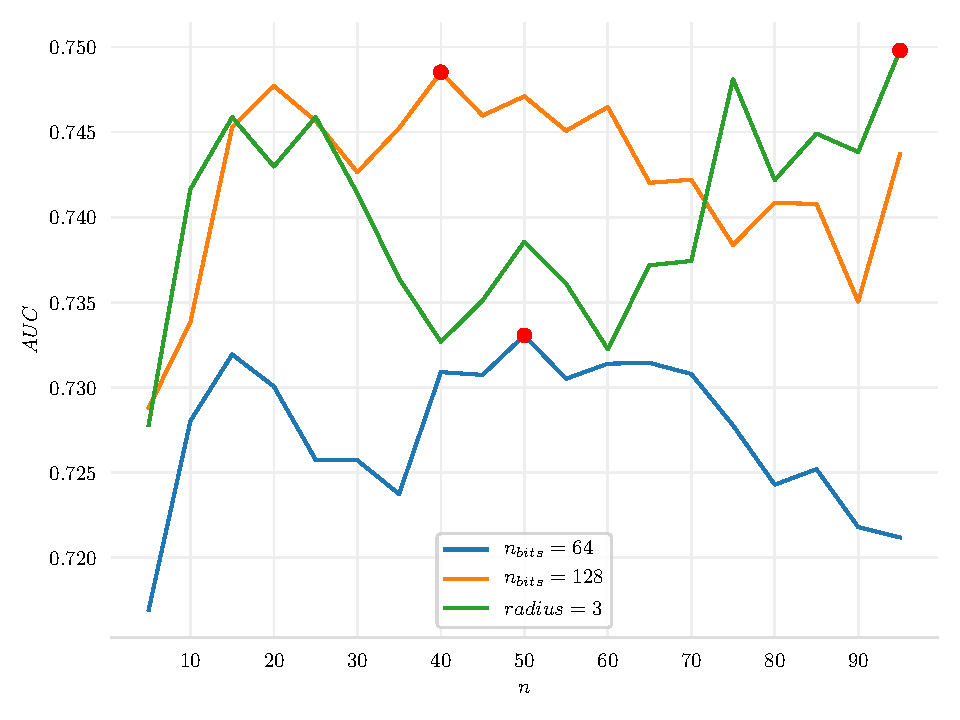
\includegraphics[width=\textwidth]{resources/pdf/knn-default-weight.pdf}
        \caption{Uniform weights}
    \end{subfigure}
    \begin{subfigure}{0.49\textwidth}
        \centering
        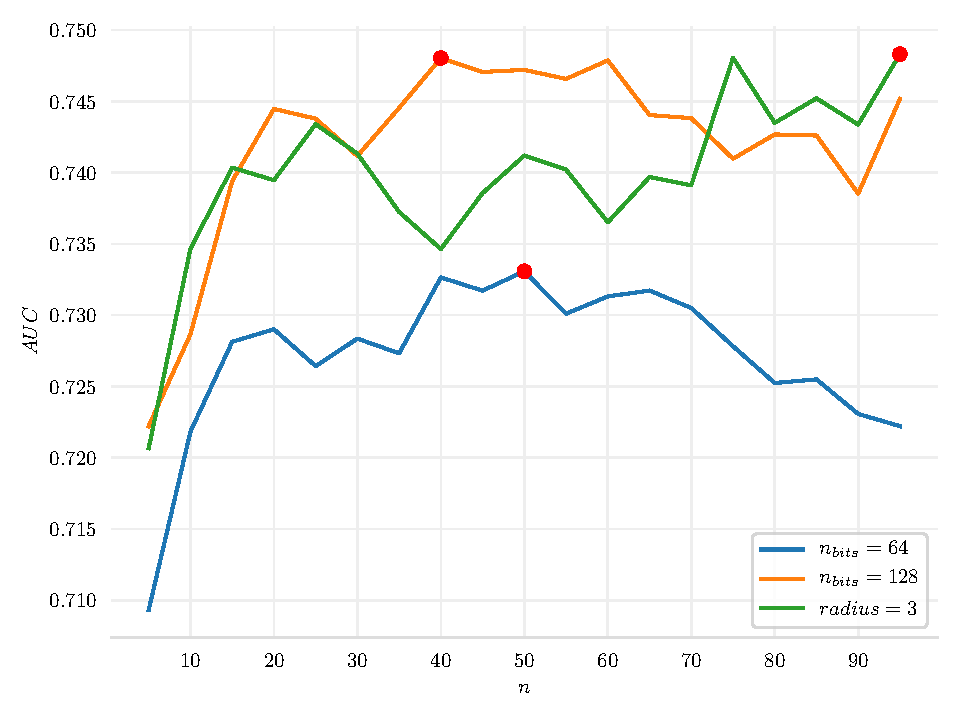
\includegraphics[width=\textwidth]{resources/pdf/knn-distance-weight.pdf}
        \caption{Anti-proportional weights}
    \end{subfigure}
    \caption{AUC estimation for KNN w.r.t. the numbers of neighbors.}
    \label{fig:knn_weight}
\end{figure}

\begin{figure}[h]
    \centering
    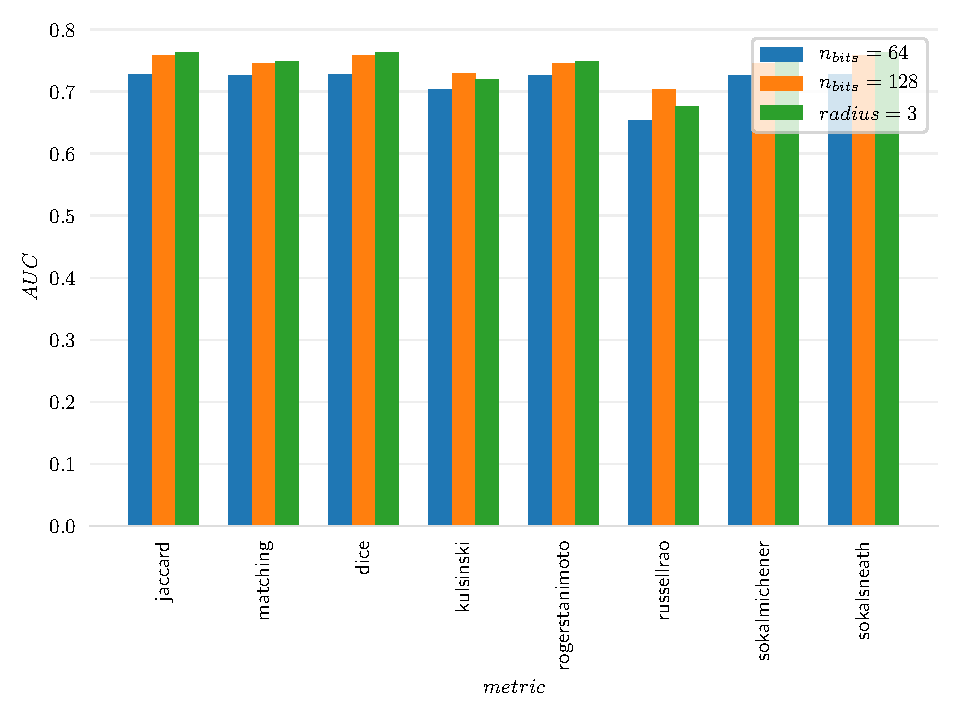
\includegraphics[width=0.59\textwidth]{resources/pdf/knn-metrics.pdf}
    \caption{AUC estimation for KNN w.r.t. the distance metric. (uniform weights and 20 neighbors)}
    \label{fig:knn_metrics}
\end{figure}

As one can see in Figures \ref{fig:knn_weight}, the uniform weights have the upper hand when fewer ($< 40$) neighbors are considered but it is the opposite afterwards, yet very slightly. By simplicity, we selected the uniform weights with $20$ neighbors which seemed a fine choice.

Concerning the metrics, it seems that none of them is significantly better than the default one. Once more by simplicity, we sticked to the default one.

What we can see, however, is that a greater number of bits induces better predictions. As stated above, this observation was made only at the end of the challenge, when we tried other fingerprints (increasing the number of bits with morgan did not provide better results for all models tested). If we had to provide another model, we would obviously increase \texttt{nBits} and use another fingerprint, as it would provide better results than the models we have designed.

\subsection{Multilayer perceptron}

The main elements of this method are the hidden layers shape and the activation function. We experienced a lot with the former and only a few with the latter. Indeed, changing the activation function for \texttt{'relu'} (default) to anything else seemed to worsen the results. We therefore varied the number of neurons per layer and the number of layers only.

\begin{figure}[h]
    \begin{subfigure}{0.49\textwidth}
        \centering
        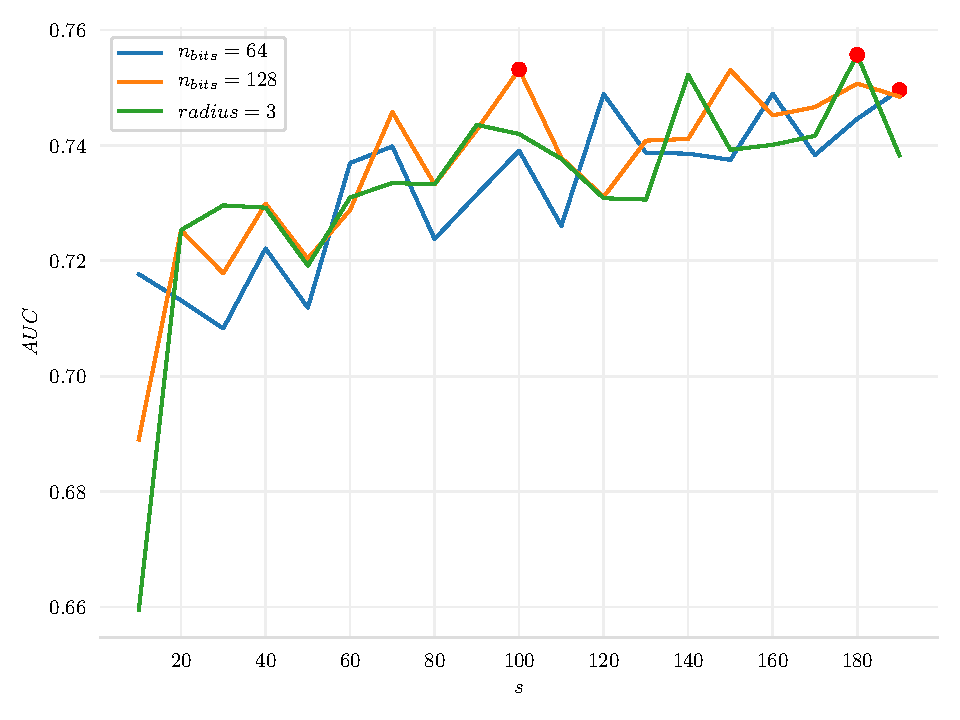
\includegraphics[width=\textwidth]{resources/pdf/mlp-layer-size.pdf}
        \caption{Number of neurons (1 layer)}
    \end{subfigure}
    \begin{subfigure}{0.49\textwidth}
        \centering
        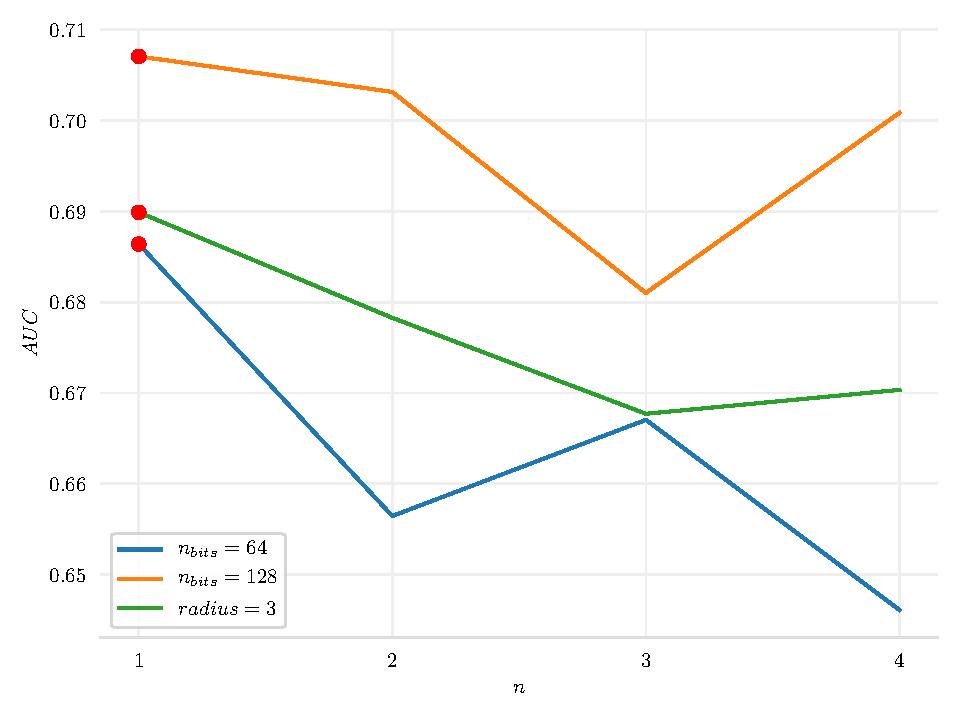
\includegraphics[width=\textwidth]{resources/pdf/mlp-layer-number.pdf}
        \caption{Number of layers (16 neurons per layer)}
    \end{subfigure}
    \caption{AUC estimation for MLP w.r.t. the shape of hidden layers.}
    \label{fig:mlp}
\end{figure}

Concerning the number of layers, it can be seen that the increase in the number of layers quickly degrades the score. A single layer seems to provide the best result. This is probably due to overfitting.

Concerning the number of neurons in the first layer, the score increases almost identically with all 3 Morgan fingerprints. A number of neurons between 100 and 200 seems to provide the best results.

\subsection{Random forest classifier}

The main parameter of this classifier is the number of trees in the forest. We therefore varied it while leaving the other parameters at their default values.

\begin{figure}[h]
    \begin{subfigure}{0.49\textwidth}
        \centering
        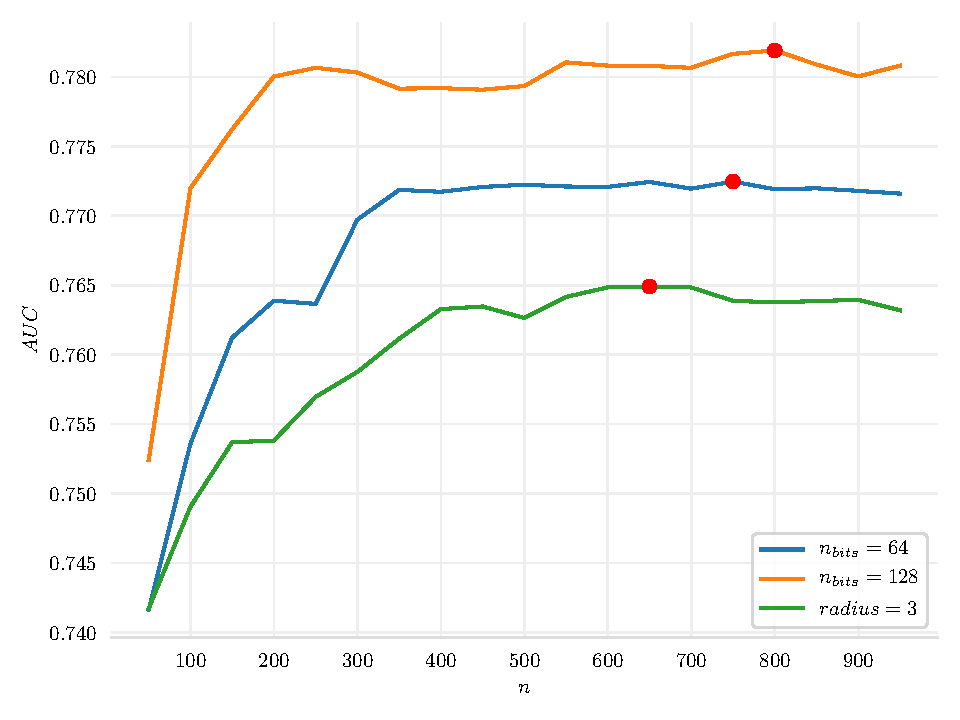
\includegraphics[width=\textwidth]{resources/pdf/rfc-number-trees.pdf}
        \caption{Unbalanced class weights}
    \end{subfigure}
    \begin{subfigure}{0.49\textwidth}
        \centering
        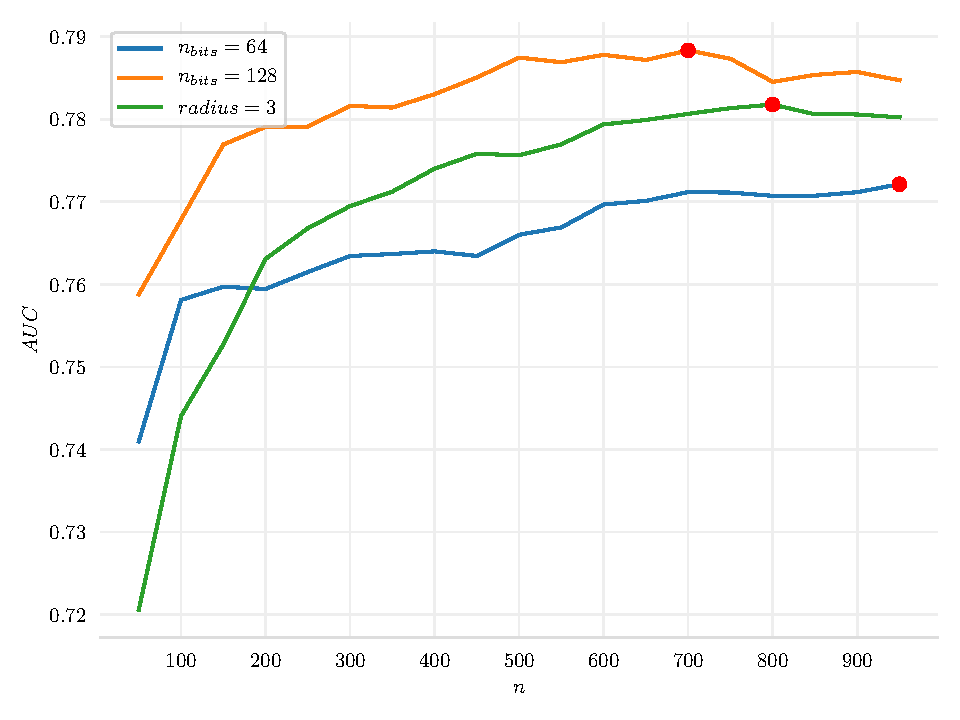
\includegraphics[width=\textwidth]{resources/pdf/rfc-number-trees-balanced.pdf}
        \caption{Balanced class weights}
    \end{subfigure}
    \caption{AUC estimation for RFC w.r.t. the number of trees.}
    \label{fig:rfc}
\end{figure}

In both cases (unbalanced and balanced class weights), the ROC AUC score appears to increase rapidly for a small number of trees and stabilizes when it increases.

In the unbalanced case, the score seems to stabilize at around 400 trees in the forest. There is a marked difference between the different parameters values for the Morgan fingerprint. The best result is, by far, obtained with 128 bits.

In the balanced case, the score stabilize later around 800 trees in the forest. The difference between fingerprint parameters is, in this case, less marked.

In both cases, the best score is obtain with Morgan using 128 bits. The score is slightly better in the balanced class weights case but the difference is very minimal.

\subsection{Support vector machine}

The main parameter of SVM is the kernel. Different kernels can deliver completely different predictions and each of them isn't suited to any problem. Therefore, we have implemented a few kernels inspired from the literature.

\begin{figure}[h]
    \centering
    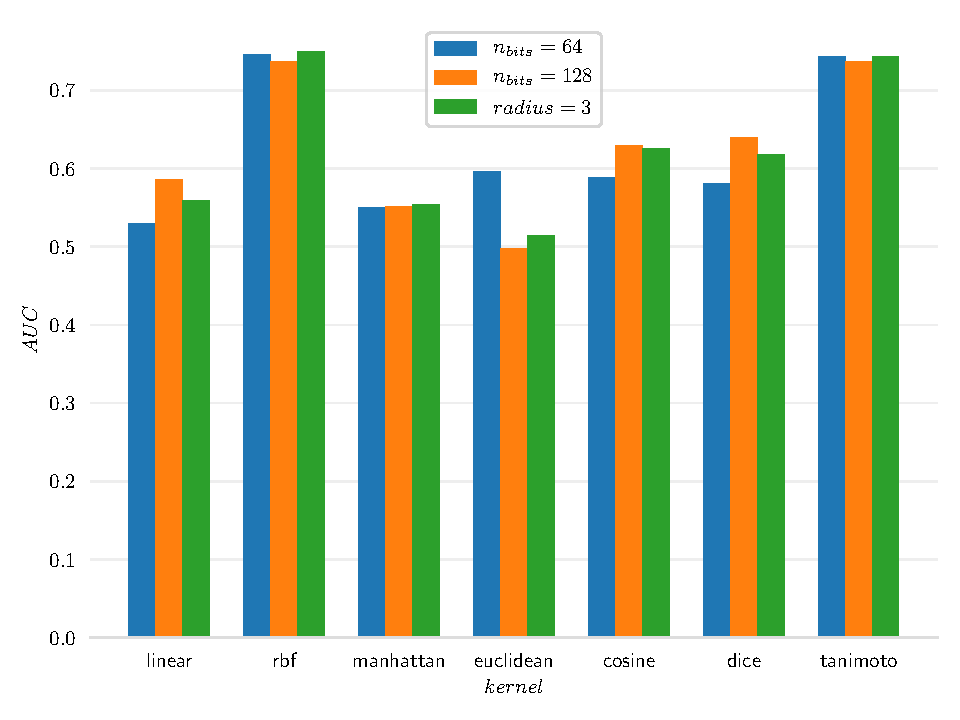
\includegraphics[width=0.66\textwidth]{resources/pdf/svm-kernels.pdf}
    \caption{AUC estimation for SVM w.r.t. the kernel.}
\end{figure}

As one can see, two kernels are largely above the others : the radial basis function (\texttt{rbf}) and the Tanimoto Similarity (\texttt{tanimoto}). Since \texttt{rbf} has one more tweaking parameter (\texttt{gamma}) than \texttt{tanimoto}, we chose it.

The other parameter of SVM is $C$, the regularization parameter. We can clearly see in the Figure \ref{fig:svm-c} that it has no influence on the predicted AUC.

\begin{figure}[h]
    \centering
    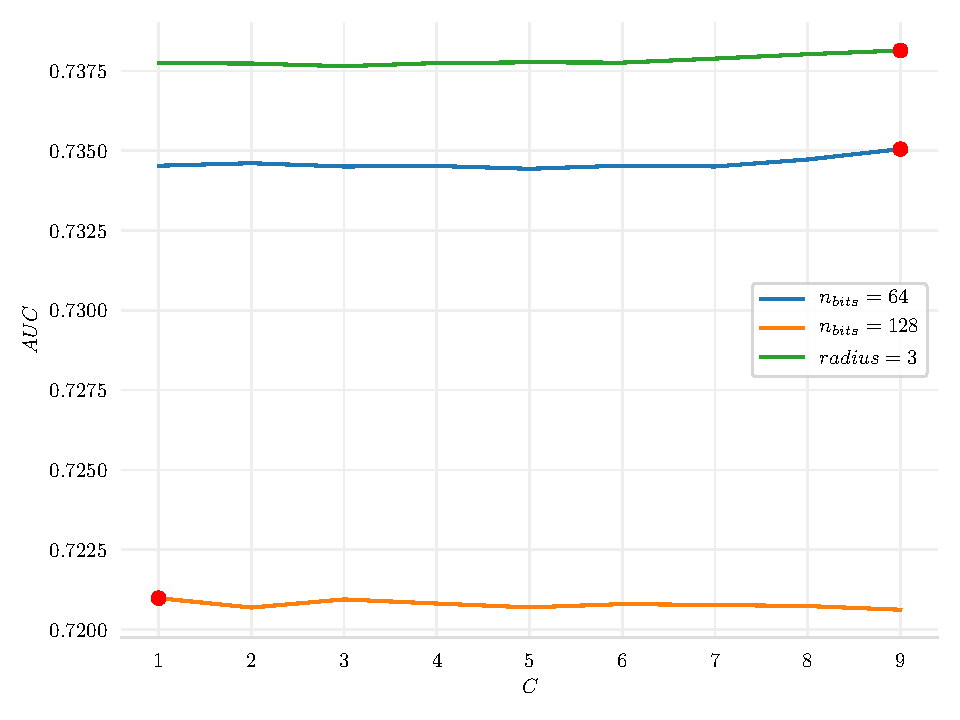
\includegraphics[width=0.66\textwidth]{resources/pdf/svm-c.pdf}
    \caption{AUC estimation for SVM w.r.t. $C$.}
    \label{fig:svm-c}
\end{figure}

\subsection{Ensemble models}

After testing some models individually in order to get an idea of their performance and the influence of their parameters on it, we tried to combine the best of them together.

The first way we tried was simply by averaging the probabilities of a set of chosen classifiers. This was done through the \texttt{VotingClassifier} of Scikit.

We also tried the \texttt{StackingClassifier} of mlxtend. This classifier doesn't average the probabilites, instead it trains another classifier (\texttt{meta\_classifier}) with the produced probabilities as input.

Finally, we designed our own ensemble classifier \texttt{ConsensusClassifier} which, as the two before, takes a list of unfitted classifiers as argument. However, instead of averaging the probabilities like the \texttt{VotingClassifier}, it computes the probability that a majority of classifier will vote \og{}in favour\fg{}.

Mathematically, we have a set $N$ of $n$ independent Bernoulli random variables $\mathcal{V}_i$ and their success probability $p_i$. Let $x$ be the number of successful variables $\mathcal{V}_i$. We have,
\begin{align*}
    P(x \geq j) & = \sum_{k = j}^{n} P(x = k) \\
    & = \sum_{k = j}^{n} \rbk{ \sum_{M \, \in \, C^k_N} P(\mathcal{V}_i = 1, \forall \, \mathcal{V}_i \in M) P(\mathcal{V}_i = 0,  \forall \, \mathcal{V}_i \in N \setminus M)} \\
    & = \sum_{k = j}^{n} \rbk{ \sum_{M \, \in \, C^k_N} \prod_{i \, \in \, M} p_i \prod_{i \, \in \, N \setminus M} (1 - p_i) }
\end{align*}
where $C^k_N$ represents the set of all $k$-combinations in $N$. Therefore, the probability computed by \texttt{ConsensusClassifier} is $$P\rbk{x \geq \frac{n + (n \bmod 2)}{2}} \, .$$

This model provides better results on our data than the two stated above, which is why this is the one we decided to keep for the tests and the final submission.

\subsection{Model Validation Technique}

In order to evaluate our models and decide if one was better than another, we decided to rely first on our prediction of the AUC. However, as these were not necessarily reflective of the score obtained on the public leaderboard, that score itself also played a role in our choices.

For example, for the submission \texttt{RFC(n\_estimators=500)} with \textit{MACCS} fingerprint (cf. Table \ref{tab:performance.summary}), we obtained an AUC estimation of \num{0.79} but a public score of \num{0.71}. We therefore decided to not investigate that fingerprint further, although the private score actually was \num{0.79} as well.

Retrospectively, we could have used other metrics to determine which model was better than another, and not base our decision only on the estimated AUC and the public score. As the public AUC was estimated from only one third of the test set, it could not be very reliable, as the classification problem was unbalanced.

The final models chosen are given at the end of the report.

	
	% ----- Fingerprints ----- %
	\section{Fingerprints}\label{sec:fingerprint}
Feature engineering is the process by which we use knowledge about the problem we face (here, the ability for a chemical compound to inhibit HIV replication) in order to create features that make machine learning efficient. As no member of the group had any knowledge about the domain, we relied on the RDKit library for Python. Given in that library are several fingerprinting methods, which identify and hash topological paths in molecules and use them to set bits in a fingerprints of user-specified lengths (taken from the RDKit documentation).

As explained in the introduction, we tried \textit{Morgan}, \textit{RDKFingerprint}, \textit{Avalon} and \textit{MACCS} fingerprints. Although we started using different fingerprints late in the challenge, we had time to test them on some submissions and found out that, in these tests, \textit{Morgan} provided better results, although the variation in scores was not very high. However, when comparing the scores obtained on the private leaderboard, it was clear that \textit{MACCS} performed better, leading to \num{0.05} increase in most models in which it had been tested, while the models tested with \textit{Morgan} that performed well on the public leaderboard provided worse results in general in the private one. This may come from the fact that the dataset used for the public leaderboard was not very representative of the whole dataset.

When testing a model (a consensus model containing KNN, MLP, SVM and RFC) with \textit{Avalon} and \num{512} bits for the fingerprinting, we reached a public score of \num{0.7564} and a private score of \num{0.8116}. Testing the same submission and only changing \textit{avalon} with \textit{Morgan} gives us a public score of \num{0.7678} and a private one of \num{0.7950}. We can see that \textit{Morgan} performed better on the \og{}public dataset\fg{}, all other things being equal, and worse on the private one than \textit{avalon}. As we based our iterative search for the best model partly on the score obtained on the public leaderboard, this is the reason we stuck with \textit{Morgan}, although the estimated AUC was almost \num{0.02} less for \textit{Morgan}.

	
	% ----- Performance summary ----- %
	\section{Performance summary} \label{sec:performance}

The table \ref{tab:performance.summary} shows the performance of different models tested. Each model was evaluated according to several scores :
\begin{itemize}
    \item $AUC_{pred}$, the score that we personally calculated;
    \item $AUC_{publ}$, the public score obtained on the Kaggle platform;
    \item $AUC_{priv}$, the private score obtained on the Kaggle platform;
    \item $VS$, the validation score, calculated as follow :
    $$
    VS = AUC_{priv} - \left | AUC_{pred} - AUC_{priv} \right |
    $$
\end{itemize}
\begin{table}[H]
    \centering
    \resizebox{0.8\textwidth}{!}{%
    \begin{tabular}{|p{4cm}|p{5cm}|c|c|c|c|}
    	\hline
    	\multirow{2}{*}{Fingerprint}                                                  & \multirow{2}{*}{Model}                        &         \multicolumn{3}{c|}{$AUC$}              & \multirow{2}{*}{$VS$}    \\ \cline{3-5}
    	                                                                              &                                               &     $pred$   &  $publ$        &     $priv$      &              \\ \hline\hline
    	\multirow{4}{4cm}{\texttt{Morgan(radius=2, nBits=128, useFeatures=False)}}    & \texttt{KNN(n\_neighbors=20)}                 & \num{0.7417} & \num{0.7062}   & \num{0.7494}    & \num{0.7417} \\ \cline{2-6}
    	                                                                              & \texttt{MLP(layers\_sizes=(100,))}            & \num{0.7449} & \num{0.7217}   & \num{0.7512}    & \num{0.7449} \\ \cline{2-6}
    	                                                                              & \texttt{SVM(kernel='rbf', gamma='auto', C=1)} & \num{0.7334} & \num{0.7027}   & \num{0.7418}    & \num{0.7334} \\ \cline{2-6}
    	                                                                              & \texttt{RFC(n\_estimators=500)}               & \num{0.7510} & \num{0.7415}   & \num{0.7827}    & \num{0.7510} \\ \hline\hline
    	\multirow{4}{4cm}{\texttt{Morgan(radius=2, nBits=128, useFeatures=True)}}     & \texttt{KNN(n\_neighbors=20)}                 & \num{0.7477} & \num{0.7469}   & \num{0.7547}    & \num{0.7477} \\ \cline{2-6}
    	                                                                              & \texttt{MLP(layers\_sizes=(100,))}            & \num{0.7531} & \num{0.7342}   & \num{0.7289}    & \num{0.7047} \\ \cline{2-6}
    	                                                                              & \texttt{SVM(kernel='rbf', gamma='auto', C=1)} & \num{0.7209} & \num{0.7536}   & \num{0.7250}    & \num{0.7209} \\ \cline{2-6}
    	                                                                              & \texttt{RFC(n\_estimators=500)}               & \num{0.7793} & \num{0.7745}   & \num{0.7758}    & \num{0.7723} \\ \cline{2-6}
    	                                                                              & \texttt{RFC(n\_estimators=500, class\_weight='balanced')} & \num{0.7874} & \num{0.7798} & \num{0.7776} & \num{0.7678} \\ \cline{2-6}
    	                                                                              & \texttt{ConsensusClassifier(\footnotemark[1])} & \num{0.7813} & \num{0.8007} & \num{0.7784} & \num{0.7755}‬  \\ \cline{2-6}
    	                                                                              & \rowcolor{blue!25} \texttt{ConsensusClassifier(\footnotemark[2])} & \num{0.7829} & \num{0.8034} & \num{0.7754} & \num{0.7679}‬ \\ \cline{2-6}
    	                                                                              & \texttt{VotingClassifier(\footnotemark[1])}    & \num{0.7823} & \num{0.7953} & \num{0.7769} & \num{0.7715} \\ \cline{2-6}
    	                                                                              & \texttt{StackingClassifier(\footnotemark[1], meta\_classifier= MLP(layers\_sizes=(100,)))}  & \num{0.7886} & \num{0.7825} & \num{0.7771} & \num{0.7656} \\ \cline{2-6}
    	                                                                              & \rowcolor{blue!25} \texttt{RFC(n\_estimators=100)}\footnotemark[3] & \num{0.7860} & \num{0.7936} & \num{0.7918} & \num{0.7860} \\ \hline\hline
    	\multirow{3}{4cm}{\texttt{MACCS()}}                                           & \texttt{KNN(n\_neighbors=20)}                 & \num{0.7468} & \num{0.7372} & \num{0.7739} & \num{0.7468} \\ \cline{2-6}
    	                                                                              & \texttt{MLP(layers\_sizes=(100,))}            & \num{0.7384} & \num{0.7479} & \num{0.7603} & \num{0.7384} \\ \cline{2-6}
    	                                                                              & \texttt{RFC(n\_estimators=500)}               & \num{0.7918} & \num{0.7154} & \num{0.7903} & \num{0.7888} \\ \hline\hline
        \texttt{Morgan(radius=2, nBits=512, useFeatures=True)}                        & \texttt{ConsensusClassifier(\footnotemark[2])} & \num{0.7690} & \num{0.7678} & \num{0.7950} & \num{0.7690}  \\ \hline
    	\texttt{Avalon(nBits=512)}                                                    & \texttt{ConsensusClassifier(\footnotemark[2])} & \num{0.7875} & \num{0.7564} & \num{0.8116} & \num{0.7875}  \\ \hline 
    	\texttt{Avalon(nBits=128)}                                                    & \texttt{ConsensusClassifier(\footnotemark[2])} & \num{0.7598} & \num{0.7281} & \num{0.7905} & \num{0.7598}  \\ \hline 
    \end{tabular}}
    \caption{Performance summary of the different models (not exhaustive)}
    \label{tab:performance.summary}
\end{table}

\footnotetext[1]{\texttt{[KNN(n\_neighbors=20), MLP(layers\_sizes=(100,)), SVM(kernel='rbf', gamma='auto', C=1), RFC(n\_estimators=500)]}}
\footnotetext[2]{\texttt{[KNN(n\_neighbors=17), MLP(layers\_sizes=(100,)), SVM(kernel='rbf', gamma='auto', C=1), RFC(n\_estimators=500)]}}
\footnotetext[3]{That model hasn't been trained with the whole learning set. Indeed, since the learning set was large (enough) but very unbalanced class-wise, we tried to counterbalance it by removing part ($\frac{6}{7}$) of the inactive components.}

\subsection{Final models selected}

The two models we selected as our \og{}final\fg{} models are the one in blue in the Table \ref{tab:performance.summary}.

\begin{enumerate}
    \item The first one is a \texttt{ConsensusClassifier}, the ensemble classifier we handcrafted. It is has been used with four classifiers : \texttt{KNN(n\_neighbors=17)}, \texttt{MLP(layers\_sizes=(100,))}, \texttt{SVM(kernel='rbf', gamma='auto', C=1)} and \texttt{RFC(n\_estimators=500)}. We chose this classifier for two reasons : 1. it was our best public submission and one of the best in our predictions; 2. because we built it ourselves, we were thrilled to see it perform better than other pre-implemented ensemble classifiers. Unfortunately, by comparing the predicted AUC (and the public score) with the private score, we deduce that this model was probably slightly overfitting the public data.
    \item The second one is a Random Forest Classifier with 100 estimators. However, as explained before\footnotemark[3], this model hasn't been trained with the whole learning. As a result, this model is less likely to overfit and the computation (fitting) time decreased dramatically. Yet, it was one of our best submission both for the AUC prediction and the public score. We therefore preferred it over slightly better models since it was one of the simplest, certainly the quickest to train and, as the main reason, because it probably overfitted less the public dataset than other models. Indeed, we can see on the final results that it was probably correct as the two scores (public and private) do not differ much.
\end{enumerate}

	
	% ----- Conclusion ----- %
	\section{Conclusion}
This project allowed us to review and apply many of the concepts seen in class, mainly the use of supervised learning techniques and the evaluation of their performance.

We also had the opportunity to investigate models that were not seen in class, as well as to get information in scientific research papers.

Although our selected models performed quite well on the public leaderboard (with AUC of $0.79360$ and $0.80340$), we found out that they underperformed on the private one, while some models that we rejected due to their low scores on the public leaderboard showed very good performance on the private one. The fact that our \textit{ConsensusClassifier} underperformed probably comes from the fact that it overfits the data used to estimate the public score. Indeed, some of the models we rejected show a score of more than $0.8$, which is better than both models we chose to be evaluated, but a public score of $0.75-0.76$.

Were we to select a new model to evaluate, we would also make sure that the number of bits used for fingerprinting is higher than what we used in our submitted models (128 bits), as the higher that number, the more complex the feature that can be detected, and we would also base our selection of algorithms on our predicted AUC without paying much attention to the public score, as our prediction was usually more reliable in that regards (as we realized \textit{a posteriori}). Indeed, some models discarded early due to their low public score had a high predicted score of more than $0.79$ and provided more than $0.80$ on the private leaderboard (simple Random Forest Classifiers with 500 or 1000 trees for example), although they showed a public score of $0.75-0.76$.

	
	% ----- Appendix ----- %
	\newpage
\appendix
\section{Code organization}
Our code consists of 6 files :
\begin{itemize}
    \item \texttt{chart.py} : this file contains customised plots functions in order to best present our results.
    \item \texttt{fingerprints.py} : this file contains several functions allowing us to test different fingerprints.
    \item \texttt{kernels.py} : this file contains several personal kernel implementations.
    \item \texttt{main.py} : this file is the main file of our code. It retrieves the data from the training set, instantiates and trains the models, evaluates their performance and creates the submission file.
    \item \texttt{models.py} : this file contains the implementation of all our models. Each model is represented by a class.
    \item \texttt{utils.py} : this file contains the various functions of our code. These functions, allowing to read CSV files, convert SMILES representations into fingerprints and create the submission file, have been taken from the toy submission proposed on the Kaggle platform.
\end{itemize}

	
	% ----- References ----- %
    \newpage
    \nocite{*}
    \printbibliography
\end{document}
